\documentclass[border=8pt]{standalone}
\usepackage{fontspec}
\setmainfont{Carlito}
\usepackage{unicode-math}
\setmathfont{Latin Modern Math}
\usepackage{xcolor}
\usepackage{pgfplots}
\pgfplotsset{compat=1.18}
\usetikzlibrary{positioning}

\definecolor{canvabg}{RGB}{246,244,241}
\pagecolor{canvabg}
\begin{document}
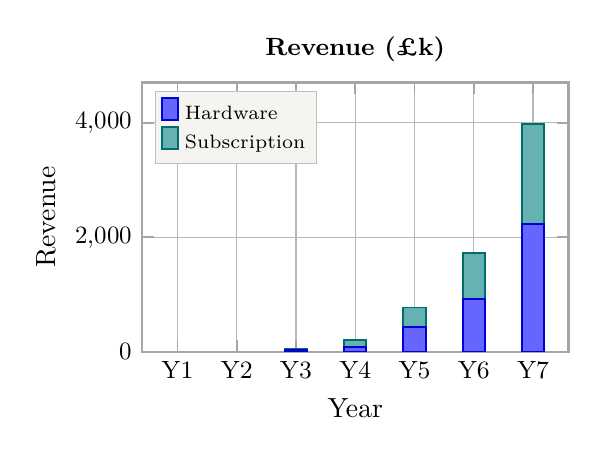
\begin{tikzpicture}
    \begin{axis}[
        width=7cm,
        height=5cm,
        symbolic x coords={Y1,Y2,Y3,Y4,Y5,Y6,Y7},
        xtick=data,
        xlabel={Year},
        grid=major,
        grid style={line width=.3pt, draw=gray!45},
        major grid style={line width=.4pt, draw=gray!55},
        axis line style={line width=0.9pt, draw=gray!70},
        tick style={line width=0.7pt, color=gray!70},
        tick label style={font=\small},
        label style={font=\normalsize},
        title style={font=\small\bfseries, yshift=-2pt},
        legend style={
            font=\scriptsize,
            cells={anchor=west},
            inner sep=2pt,
            row sep=-1pt,
            fill=canvabg,
            draw=gray!50,
        },
        title={Revenue (\pounds k)},
        ylabel={Revenue},
        ybar stacked,
        bar width=8pt,
        ymin=0, ymax=4700,
        legend pos=north west,
        legend columns=1,
    ]
    \addplot+[ybar,fill=blue!60,draw=blue!85!black,line width=0.7pt] coordinates {(Y1,0.0) (Y2,0.0) (Y3,26.5) (Y4,79.4) (Y5,438.4) (Y6,927.3) (Y7,2227.1)};
    \addplot+[ybar,fill=teal!60,draw=teal!85!black,line width=0.7pt] coordinates {(Y1,0.0) (Y2,0.0) (Y3,27.0) (Y4,132.3) (Y5,335.1) (Y6,796.6) (Y7,1751.9)};
    \legend{Hardware, Subscription}
    \end{axis}
\end{tikzpicture}
\end{document}
